\documentclass[10pt,twocolumn]{article}

\usepackage[margin=0.75in, top=1in, bottom=1in]{geometry}
\usepackage{amsmath,amsfonts,amssymb}
\usepackage{graphicx}
\usepackage{float}
\usepackage{tikz}
\usetikzlibrary{arrows.meta,positioning,fit,calc}
\usepackage{xcolor}
\usepackage{caption}
\usepackage{booktabs}
\usepackage{hyperref}
\usepackage{titlesec}
\usepackage{abstract}
\usepackage{parskip}
\usepackage{fancyhdr}

\titleformat{\section}{\normalfont\large\bfseries\scshape}{{\Roman{section}.}}{0.5em}{}
\titleformat{\subsection}{\normalfont\normalsize\bfseries\itshape}{{\Alph{subsection}.}}{0.4em}{}
\titlespacing*{\section}{0pt}{8pt}{4pt}
\titlespacing*{\subsection}{0pt}{6pt}{2pt}

\tikzset{
  block/.style={draw, rounded corners=2pt, align=center, minimum width=1.25cm,
                minimum height=0.5cm, font=\tiny, fill=blue!6, thick},
  dev/.style={draw, rounded corners=2pt, align=center, minimum width=1.15cm,
              minimum height=0.48cm, font=\tiny, fill=orange!10},
  arrow/.style={-Stealth, semithick, gray!70!black},
}

\pagestyle{fancy}
\fancyhf{}
\rhead{\small Distributed Motion Tracker}
\lhead{\small Rousseau \& Nwabueze --- USC}
\cfoot{\thepage}
\renewcommand{\headrulewidth}{0.4pt}

\begin{document}

\twocolumn[{
\begin{@twocolumnfalse}
  \begin{center}
    {\LARGE\bfseries Distributed Motion Sensing for Web Visualization and Air-Painting}\\[6pt]
    {\large Kamron Rousseau \quad Kamsi Nwabueze}\\[2pt]
    {\normalsize Dept.\ of Electrical and Computer Engineering, University of Southern California}\\[2pt]
    {\normalsize Los Angeles, CA~90089}\\[8pt]
  \end{center}
  \begin{abstract}
    \noindent
    We built a small networked system where ESP32 nodes stream sensor data over WiFi to a Python
    server on a laptop, which fuses or forwards measurements and pushes updates to a browser over
    WebSocket. One application is a tilt-driven air-paint canvas with ultrasonic gestures (pen lift
    near the sensor, swipe-to-undo from speed). The other is a live 3D block and motion trail driven
    by inertial data, with camera zoom from ultrasonic range. The motion node reads two inertial
    sensors on a shared I\textsuperscript{2}C bus at distinct addresses; the paint node reads a
    single MPU over I\textsuperscript{2}C. The ultrasonic module (HC-SR04) is powered from 5\,V;
    its ECHO output is level-shifted with a resistor divider before GPIO~18 because ECHO swings to
    5\,V while the ESP32 inputs are 3.3\,V-rated.
  \end{abstract}
  \vspace{8pt}
\end{@twocolumnfalse}
}]

\section{Introduction}

The goal was to split sensing across ESP32 ``nodes'' and centralize visualization on a laptop.
Each node connects to WiFi, opens a TCP socket to the host, and sends newline-delimited JSON at
roughly tens of hertz. Two Python entry points serve different demos: \texttt{server.py} (block
viewer, ports 9001/9002, browser on 5001) and \texttt{paint\_server.py} (canvas, ports 9000/9002,
browser on 5002). Only one of these should own TCP~9002 if a single ultrasonic board is used.

\section{System Block Diagram}

Figure~\ref{fig:block} summarizes data flow. The diagram is intentionally compact: all edge
traffic is JSON over TCP; the host repackages into Socket.IO events for the browser.

\begin{figure}[H]
\centering
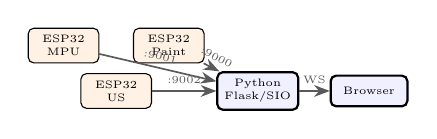
\begin{tikzpicture}[scale=0.78, transform shape,
                    node distance=0.35cm and 0.4cm, font=\tiny]
  \node[dev] (imu) {ESP32\\MPU};
  \node[dev, right=0.55cm of imu] (paint) {ESP32\\Paint};
  \node[dev, below=0.45cm of $(imu)!0.5!(paint)$] (us) {ESP32\\US};
  \node[block, right=1.05cm of us] (py) {Python\\Flask/SIO};
  \node[block, right=0.5cm of py] (web) {Browser};

  \draw[arrow] (imu) -- node[above,sloped,font=\tiny]{:9001} (py);
  \draw[arrow] (paint) -- node[above,sloped,font=\tiny]{:9000} (py);
  \draw[arrow] (us) -- node[above,font=\tiny]{:9002} (py);
  \draw[arrow] (py) -- node[above,font=\tiny]{WS} (web);
\end{tikzpicture}
\caption{High-level data flow (WiFi end-to-end). TCP: newline JSON. Browser: Socket.IO $\approx$20\,Hz.}
\label{fig:block}
\end{figure}

\section{Components and Design Choices}

\subsection{Inertial sensing (I\textsuperscript{2}C)}

On the \textbf{motion} ESP32, two MPU9250-class devices share one I\textsuperscript{2}C bus
(SDA/SCL) at different 7-bit addresses (0x68 and 0x69) by wiring AD0 low on one unit and high on
the other. Reads use the Arduino \texttt{Wire} API with register bursts for accelerometer and gyro
data; orientation-style quantities are computed or forwarded for fusion on the host. Bus clock is
kept moderate (100\,kHz) for robustness on jumper wires.

The \textbf{paint} ESP32 uses a single MPU6050/compatible IMU on the same bus (address 0x69 in
our wiring). Roll and pitch drive cursor velocity on the canvas after a simple bias calibration
in the page.

\subsection{Ultrasonic ranging}

An HC-SR04 measures round-trip time on ECHO. VCC is 5\,V (module spec); TRIG is driven from a
3.3\,V GPIO output, which the module accepts. ECHO returns a 5\,V pulse, so we do \emph{not} connect
ECHO directly to the ESP32: a two-resistor divider (e.g.\ 1\,k$\Omega$ upper, 2\,k$\Omega$ lower to
ground) feeds GPIO~18 with $\approx$\,3.3\,V high level. Firmware uses a GPIO interrupt on ECHO (both
edges) to timestamp the pulse width instead of blocking \texttt{pulseIn}. On-node filtering uses a
short sliding window mean plus a startup baseline for relative distance and a finite-difference
speed estimate for gesture events.

\subsection{Host and transport}

TCP is plain text, one JSON object per line, which keeps the ESP32 side simple. Flask-SocketIO
broadcasts fused or raw fields at about 20\,Hz so the UI stays light. For the 3D view, fusion maps
tilt-derived quantities to position for the trail; for paint, the server merges MPU and ultrasonic
streams into one WebSocket payload when both TCP clients are connected. Reconnect loops on the
ESP32 tolerate the server being down during boot.

\section{Ultrasonic front-end schematic}

Figure~\ref{fig:sch} shows the interface between the HC-SR04 and the ESP32 ultrasonic node.
TRIG connects directly to GPIO~5 (3.3\,V output). The divider scales the 5\,V ECHO high level to
$V_{\mathrm{GPIO}} \approx 5\,\mathrm{V}\times\frac{R_2}{R_1+R_2}\approx 3.3$\,V at the tap when
$R_1=1$\,k$\Omega$ and $R_2=2$\,k$\Omega$. All grounds must be tied together.

\begin{figure}[H]
\centering
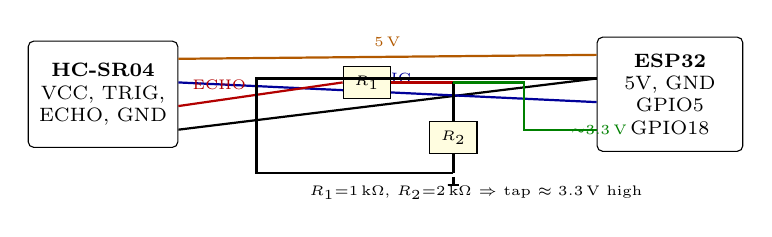
\begin{tikzpicture}[font=\scriptsize]
  % HC-SR04
  \node[draw, rounded corners=2pt, minimum width=1.9cm, minimum height=1.35cm, align=center] (sr)
    at (0,0) {\textbf{HC-SR04}\\VCC, TRIG,\\ECHO, GND};
  % ESP32
  \node[draw, rounded corners=2pt, minimum width=1.85cm, minimum height=1.45cm, align=center] (esp)
    at (7.2,0) {\textbf{ESP32}\\5V, GND\\GPIO5\\GPIO18};

  % Anchor points on box edges
  \coordinate (srV)  at ($(sr.east)+(0,0.45)$);
  \coordinate (srT)  at ($(sr.east)+(0,0.15)$);
  \coordinate (srE)  at ($(sr.east)+(0,-0.15)$);
  \coordinate (srG)  at ($(sr.east)+(0,-0.45)$);

  \coordinate (esp5) at ($(esp.west)+(0,0.5)$);
  \coordinate (espG) at ($(esp.west)+(0,0.2)$);
  \coordinate (espT) at ($(esp.west)+(0,-0.1)$);
  \coordinate (espE) at ($(esp.west)+(0,-0.45)$);

  % Direct wires
  \draw[thick, orange!70!black] (srV) -- node[above, font=\tiny, sloped]{5\,V} (esp5);
  \draw[thick] (srG) -- (espG);
  \draw[thick, blue!60!black] (srT) -- node[above, font=\tiny, sloped]{TRIG} (espT);

  % Divider: ECHO -> R1 -> tap -> R2 -> GND ; tap -> GPIO18
  \coordinate (tap) at (4.45,0.15);
  \coordinate (gndtap) at (4.45,-1.0);

  \node[draw, minimum width=0.6cm, minimum height=0.38cm, fill=yellow!12] (R1) at (3.35,0.15) {\tiny$R_1$};
  \node[draw, minimum width=0.6cm, minimum height=0.38cm, fill=yellow!12] (R2) at (4.45,-0.55) {\tiny$R_2$};

  \draw[thick, red!70!black] (srE) -- node[above, font=\tiny, near start]{ECHO} (R1.west);
  \draw[thick, red!70!black] (R1.east) -- (tap);
  \draw[thick] (tap) -- (R2.north);
  \draw[thick] (R2.south) -- (gndtap);
  \draw[thick] (gndtap) -- ++(-2.5,0) |- (espG);

  \draw[thick, green!50!black] (tap) -- ++(0.9,0) |- node[right, font=\tiny, pos=0.75]{$\sim$3.3\,V} (espE);

  \node[anchor=west, font=\tiny] at (2.5,-1.25)
    {$R_1{=}1$\,k$\Omega$, $R_2{=}2$\,k$\Omega$ $\Rightarrow$ tap $\approx 3.3$\,V high};

  % GND symbol at gndtap
  \draw[thick] (gndtap) ++(0,-0.05) -- ++(0,-0.1) -- ++(-0.07,0) -- ++(0.14,0);
\end{tikzpicture}
\caption{HC-SR04 to ESP32 (conceptual schematic). ECHO divider protects the 3.3\,V input; pin numbers match \texttt{ultrasonic\_node/include/config.h}.}
\label{fig:sch}
\end{figure}

\subsection{Demo and testing}

We verified WiFi/TCP paths with the Python listeners printing client connects, and exercised the
paint UI with \texttt{nc} injecting JSON on port~9002 when hardware was unavailable. Serial
logging at 115200\,baud on the ESP32s confirmed trigger/echo timing and reconnection after server
restarts. Browser devtools showed steady Socket.IO event rates near the configured 20\,Hz when
both ESP streams were live.

\section{Limitations and Lessons Learned}

\textbf{Single ultrasonic, single TCP port.} Both servers default to port~9002 for the ultrasonic
client; only one listener can bind. For demos we stop one server before starting the other, or we
would need a second port and firmware change.

\textbf{Network and timing.} WiFi jitter shows up as occasional stale UI labels; we freeze or
clamp motion when packets stop. Ultrasonic rate is limited by acoustic flight time and filtering.

\textbf{HC-SR04 behavior.} Soft targets, angles, and crosstalk cause noisy distance; thresholds
for pen lift and swipe-undo required tuning and hysteresis. Using absolute distance (cm) for
near-field pen lift behaved more predictably than startup-relative offset alone.

\textbf{I\textsuperscript{2}C layout.} Long Dupont leads increase capacitance and can cause NACKs;
keeping wires short and sharing a solid ground reference helped more than aggressive clock increases.

\textbf{Takeaway.} End-to-end contracts (JSON keys, ports, IP in \texttt{config.h}) matter as
much as the algorithms. Level-shifting ECHO is non-optional for a clean 3.3\,V GPIO design; a
dedicated level shifter IC would be even cleaner than a divider if we had to meet tight timing
margins at higher baud rates (not an issue here).

\end{document}
